% Options for packages loaded elsewhere
\PassOptionsToPackage{unicode}{hyperref}
\PassOptionsToPackage{hyphens}{url}
%
\documentclass[
]{book}
\usepackage{amsmath,amssymb}
\usepackage{lmodern}
\usepackage{iftex}
\ifPDFTeX
  \usepackage[T1]{fontenc}
  \usepackage[utf8]{inputenc}
  \usepackage{textcomp} % provide euro and other symbols
\else % if luatex or xetex
  \usepackage{unicode-math}
  \defaultfontfeatures{Scale=MatchLowercase}
  \defaultfontfeatures[\rmfamily]{Ligatures=TeX,Scale=1}
\fi
% Use upquote if available, for straight quotes in verbatim environments
\IfFileExists{upquote.sty}{\usepackage{upquote}}{}
\IfFileExists{microtype.sty}{% use microtype if available
  \usepackage[]{microtype}
  \UseMicrotypeSet[protrusion]{basicmath} % disable protrusion for tt fonts
}{}
\makeatletter
\@ifundefined{KOMAClassName}{% if non-KOMA class
  \IfFileExists{parskip.sty}{%
    \usepackage{parskip}
  }{% else
    \setlength{\parindent}{0pt}
    \setlength{\parskip}{6pt plus 2pt minus 1pt}}
}{% if KOMA class
  \KOMAoptions{parskip=half}}
\makeatother
\usepackage{xcolor}
\usepackage{longtable,booktabs,array}
\usepackage{calc} % for calculating minipage widths
% Correct order of tables after \paragraph or \subparagraph
\usepackage{etoolbox}
\makeatletter
\patchcmd\longtable{\par}{\if@noskipsec\mbox{}\fi\par}{}{}
\makeatother
% Allow footnotes in longtable head/foot
\IfFileExists{footnotehyper.sty}{\usepackage{footnotehyper}}{\usepackage{footnote}}
\makesavenoteenv{longtable}
\usepackage{graphicx}
\makeatletter
\def\maxwidth{\ifdim\Gin@nat@width>\linewidth\linewidth\else\Gin@nat@width\fi}
\def\maxheight{\ifdim\Gin@nat@height>\textheight\textheight\else\Gin@nat@height\fi}
\makeatother
% Scale images if necessary, so that they will not overflow the page
% margins by default, and it is still possible to overwrite the defaults
% using explicit options in \includegraphics[width, height, ...]{}
\setkeys{Gin}{width=\maxwidth,height=\maxheight,keepaspectratio}
% Set default figure placement to htbp
\makeatletter
\def\fps@figure{htbp}
\makeatother
\setlength{\emergencystretch}{3em} % prevent overfull lines
\providecommand{\tightlist}{%
  \setlength{\itemsep}{0pt}\setlength{\parskip}{0pt}}
\setcounter{secnumdepth}{5}
\usepackage{booktabs}
\ifLuaTeX
  \usepackage{selnolig}  % disable illegal ligatures
\fi
\usepackage[]{natbib}
\bibliographystyle{plainnat}
\IfFileExists{bookmark.sty}{\usepackage{bookmark}}{\usepackage{hyperref}}
\IfFileExists{xurl.sty}{\usepackage{xurl}}{} % add URL line breaks if available
\urlstyle{same} % disable monospaced font for URLs
\hypersetup{
  pdftitle={Inngangur að ályktunartölfræði},
  pdfauthor={Katrín Arndís},
  hidelinks,
  pdfcreator={LaTeX via pandoc}}

\title{Inngangur að ályktunartölfræði}
\author{Katrín Arndís}
\date{2023-02-11}

\begin{document}
\maketitle

{
\setcounter{tocdepth}{1}
\tableofcontents
}
\hypertarget{formuxe1li}{%
\chapter{Formáli}\label{formuxe1li}}

Í þessu skjali fer ég yfir hugtök og hugmyndir sem eru nauðsynleg
undirstaða þess að skilja þau umfjöllunarefni sem koma í framhaldinu.
Athugið að þetta er með öllu óyfirfarið efni, svo villur gætu leynst í
textanum.

\hypertarget{grunn-hugtuxf6k}{%
\section{Grunn hugtök}\label{grunn-hugtuxf6k}}

Eftirfarandi eru hugtök sem þarf að þekkja við lestur þessa skjals:

\begin{itemize}
\tightlist
\item
  \textbf{Þýði} er sá hópur sem við viljum læra eitthvað um; það getur
  endurspeglað stóran hóp einstaklinga (Evrópubúar), smærri hóp
  (Íslendingar) eða heldur lítinn hóp (nemendur HR).

  \begin{itemize}
  \tightlist
  \item
    Þýði þarf að vera skýr, afmarkaður hópur einstaklinga sem eiga
    eitthvað sameiginlegt.\footnote{Hér er talað um einstaklinga, það má þó beita
      ályktunartölfræði á hvað sem er; dýr, bíla, sveppi eða jafnvel
      hnetusmjör. Hugmyndin stendur þó: þýði endurspeglar heildina sem við
      viljum draga ályktanir um og sú heild samanstendur af stökum. Í þýði
      Íslendinga væri hver Íslendingur 1 stak.}
  \end{itemize}
\item
  \textbf{Þýðistölur} eru þau gildi sem fengjust ef við hefðum aðgang að
  öllu þýðinu.

  \begin{itemize}
  \tightlist
  \item
    Gefum okkur að við viljum vita hæð Íslendinga, það er einhver
    meðalhæð sem fengist ef \textbf{öll stök þýðis} væru mæld. Við getum
    ekki mælt \emph{alla} sem þýði samanstendur af -- við drögum því
    úrtak og athugum eiginleika úrtaksins til að komast sem næst
    raunverulegu þýðisgildi.
  \end{itemize}
\item
  \textbf{Úrtak} er sá hópur sem við mælum því við teljum hann endurspegla
  þýðið. Við reynum yfirleitt að draga með tilviljunarkenndum hætti úr
  þýði.
\item
  \textbf{Úrtakstölur} eru þau gildi sem fást frá úrtakinu. Í úrtaki
  Íslendinga fæst einhvert meðaltal fyrir hæð, þetta meðaltal er dæmi
  um úrtakstölu og er það næsta sem við komumst því að vita hver hæðin
  er í \emph{raun} (þýðinu).
\end{itemize}

\hypertarget{duxe6mi-sem-veruxf0ur-unniuxf0-meuxf0.}{%
\subsection*{Dæmi sem verður unnið með.}\label{duxe6mi-sem-veruxf0ur-unniuxf0-meuxf0.}}
\addcontentsline{toc}{subsection}{Dæmi sem verður unnið með.}

\emph{Við viljum vita hvort háskólamenntaðir fái hærri laun heldur en þau sem
hafa ekki háskólamenntun á Íslandi.}

Hér höfum við afmarkað þýði -- við erum að skoða fólk með búsetu á
Íslandi. Úr þýði Íslendinga myndum við draga úrtak og athuga menntun og
mánaðarlaun hvers einstaklings í úrtakinu. Rannsóknarspurningin er
einnig skýr en hana mætti endurorða á eftirfarandi hátt: Við viljum
athuga hvort meðal mánaðarlaun á Íslandi séu að jafnaði ólík á milli
tveggja hópa; þeirra sem hafa háskólamenntun og þeirra sem hafa hana
ekki. \footnote{Spurningin gæti þó verið sett upp á ólíkan hátt eftir því
  hvernig við kjósum að mæla breyturnar og hvaða tölfræðiaðferð við
  notum}

\hypertarget{tilguxe1tupruxf3fun}{%
\chapter{Tilgátuprófun}\label{tilguxe1tupruxf3fun}}

Þegar við framkvæmum rannsókn höfum við einhverjar spurningar í huga sem
við viljum leitast svara við. Augljóst vandamál er að tölfræðiforrit
skilja ekki setningar -- við getum ekki beinlínis sett gögn inn í
úrvinnslu ásamt spurningunni ``eru mánaðarlaun ólík eftir menntun
fólks?''.

Það mætti hugsa ferlið á eftirfarandi hátt: Við yfirfærum spurningarnar
okkar yfir á \emph{tölfræðimál} sem forritið skilur og ákveðum hvaða aðferð
eigi að nota við að svara spurningunni okkar. Forritið vinnur úr
gögnunum fyrir okkur og spýtir út niðurstöðum. Þessar niðurstöður eru þó
á \emph{tölfræðimáli} og það er okkar verk að skilja hvað þær segja okkur og
geta gefið túlkun sem setur þær aftur á \emph{mannamál}.

Í \textbf{tilgátuprófun} fáum við skýrt svar við spurningunni okkar; já eða
nei -- eftir því hvort niðurstöður reynast marktækar eða ómarktækar.

\hypertarget{cross}{%
\section{Tilgátur}\label{cross}}

Við byrjum á því að setja spurninguna okkar fram í formi \textbf{tilgátu}. Í
okkar dæmi viljum við vita hvort það sé munur á launum einstaklinga
eftir menntun viðkomandi.

\hypertarget{auxf0altilguxe1ta}{%
\subsection{Aðaltilgáta}\label{auxf0altilguxe1ta}}

\textbf{Aðaltilgáta} \footnote{Einnig kölluð gagntilgáta, rannsóknartilgáta, (e.
  alternative hypothesis)} er sú tilgáta sem við höfum áhuga
á \footnote{Undantekningar eru t.d. þegar við beitum
  marktektarprófum við mat á forsendum} og tilgreinir einhvers konar mun. Vandamálið er
að hún tilgreinir enga fasta tölu sem hægt er að prófa og því ógerlegt
að prófa hana beint.

Í okkar dæmi gæti verið munur á launum eftir menntun, en hvaða mun ætti
að prófa? Munurinn gæti verið að laun háskólamenntaðra séu 1kr hærri,
15kr, 1.000kr, 35.000kr, 645.000kr, og svo framvegis. Tilgátan ``það er
munur'' hefur svo marga möguleika að það er ekki hægt að prófa þá alla.
Við setjum því fram núlltilgátu.

\hypertarget{nuxfalltilguxe1ta}{%
\subsection{Núlltilgáta}\label{nuxfalltilguxe1ta}}

\textbf{Núlltilgáta} tilgreinir tiltekið tölugildi, þar sem \emph{ef} það tiltekna
gildi væri í raun rétt -- þá gæti aðaltilgátan ekki líka verið rétt. Í
okkar dæmi yrði núlltilgátan sú að laun séu þau sömu óháð
háskólamenntun.

Þetta er ekki það sama og að segja að \emph{allir séu með sömu laun} heldur
að þegar við berum saman meðallaun þeirra sem hafa háskólamenntun og
þeirra sem hafa hana ekki þá sé meðaltalið hið sama, munurinn = 0, það
er engin munur á meðallaunum hópana.

\begin{center}\rule{0.5\linewidth}{0.5pt}\end{center}

Ef niðurstaðan er að núlltilgátan sé röng -- þá hlýtur andstæða hennar
að vera rétt. Með öðrum orðum, ef við teljum ólíklegt að það sé
\textbf{engin} munur, þá hlýtur jú að vera munur - aðaltilgátan hlýtur þá að
vera rétt.

Nú höfum við sett fram tilgátur og næsta skref er að athuga \textbf{hvort}
við höfum rétt fyrir okkur -- til þess framkvæmum við marktektarpróf.

\hypertarget{marktekt}{%
\chapter{Marktekt}\label{marktekt}}

Þegar við skoðum úrtakið okkar gætum við séð mun á launum þeirra sem hafa og hafa ekki háskólamenntun. Tilgangur ályktunartölfræði er þó ekki \emph{spá fyrir um} úrtakið okkar -- úrtakstölurnar eru jú beint fyrir framan okkur svo lýsandi tölfræði myndi duga til að lýsa þeim. Munurinn sem við sjáum í úrtakinu okkar gæti þó verið tilkomin af hreinni tilviljun:

\begin{enumerate}
\def\labelenumi{\arabic{enumi}.}
\item
  20 manna úrtak þar sem launamunur reynist 10.000kr á milli þeirra sem hafa háskólamenntun og þeirra sem hafa ekki háskólamenntun. Í þessu úrtaki er vissulega munur en það er auðvelt að ímynda sér að hann sé ekki að endurspegla mun í þýði. Það er, að þessi 10.000kr munur sé tilviljun sem búast mætti við í smáu úrtaki.
\item
  2.000 manna úrtak þar sem launamunur reynist 100.000kr á milli hópanna. Hér þætti okkur frekar ólíklegt að svo mikill munur fyndist af tilviljun, í svo stóru úrtaki, \textbf{ef það væri engin munur á hópunum í þýði}.
\end{enumerate}

Eftir því sem munurinn er meiri og úrtakið stærra, þeim mun ólíklegra verður að þykja að úrtakstölurnar séu tilkomnar af einskærri tilviljun. Þá situr eftir sú spurning: Hversu mikill munur er nógu mikill? Og þá miðað við hversu stórt úrtak? \footnote{Það er þó auðvitað fleira sem spilar inn í útreikning marktektarprófa - þetta er einföldun.}

Marktektarpróf athugar líkur þess að fá tilteknar úrtakstölur \textbf{ef úrtakið kæmi úr þýði þar sem núlltilgátan er í raun rétt.} \emph{Ef það er í raun \textbf{enginn} munur á launum þeirra sem hafa og hafa ekki háskólamenntun, hverjar eru þá líkurnar á því að fá 100.000kr mun í úrtaki sem samanstendur af 2.000 einstaklingum?}

Ef líkurnar eru mjög litlar, þá er sömuleiðis ólíklegt að núlltilgátan sé rétt. Þegar við höfnum núlltilgátunni, þá tökum við upp aðaltilgátuna og ályktum að það sé í raun munur á hópunum í þýði.

Ef það væru hins vegar miklar líkur á úrtaksgildunum þegar það væri dregið úr þýði þar sem engin munur er, þá myndum við hika verulega við að henda fram fullyrðingum. Við færum varla að koma með staðhæfingar ef við vitum að það eru 50\% líkur á að niðurstaðan sé tilkomin af tilviljun.

Næsta spurning er þá -- hversu litlar þurfa líkurnar að vera svo við séum sátt?

\begin{center}\rule{0.5\linewidth}{0.5pt}\end{center}

\hypertarget{marktektarmuxf6rk}{%
\section{Marktektarmörk}\label{marktektarmuxf6rk}}

\textbf{Marktektarmörk} (\(\alpha\)) lýsa því einmitt hvar við drögum línuna, í sálfræði er nærri alltaf miðað við \(\alpha\)= 0,05. \footnote{Sumar fræðigreinar miða við 0,01 (ef röng ákvörðun er t.d. tekin í stjarnfræði geta afleiðingar verið miklar). Aðrar fræðigreinar, þar sem mistök eru ekki eins alvarleg, geta miðað við 0,1.} Þessi tala (0,05) vísar til líkinda (5\%) og við erum þá að segja að við viljum að það séu undir 5\% líkur á að við höfum rangt fyrir okkur. \footnote{Að hafa rangt fyrir okkur þýðir hér að við ályktum að það sé, eða sé ekki marktækur munur og að sú ákvörðun sé röng}

\hypertarget{marktektarpruxf3f}{%
\section{Marktektarpróf}\label{marktektarpruxf3f}}

\textbf{Marktektapróf} reikna líkur þess að fá tilteknar niðurstöður þegar núlltilgáta er í raun rétt og kallar þessar líkur \emph{p}-gildi. \emph{P}-gildi endurspeglar þannig líkur þess að við höfum rangt fyrir okkur. Ef við höfum ákveðið að miða við marktektarmörk = 0,05 þá munu allar niðurstöður þar sem \emph{p}-gildi er yfir 0,05 þýða að niðurstöður séu ómarktækar. \emph{P}\textgreater{} 0,05 þýðir að það séu yfir 5\% líkur á að við höfum rangt fyrir okkur og við vorum jú búin að ákveða að draga mörkin við 5\%.

Höfum samt í huga að þó 5\% séu lágar líkur, þá eru þær ekki 0\% -- svo við \emph{gætum} við haft rangt fyrir okkur. Skoðum því aðeins hvernig niðurstaða gæti verið rétt eða röng með því að gefa okkur eftirfarandi aðstæður í þýði:

\begin{longtable}[]{@{}
  >{\raggedright\arraybackslash}p{(\columnwidth - 4\tabcolsep) * \real{0.1705}}
  >{\raggedright\arraybackslash}p{(\columnwidth - 4\tabcolsep) * \real{0.4432}}
  >{\raggedright\arraybackslash}p{(\columnwidth - 4\tabcolsep) * \real{0.3864}}@{}}
\caption{Tafla 1. Mögulegar niðurstöður marktektarprófs ef við þekkjum aðstæður í þýði.}\tabularnewline
\toprule()
\endhead
& \textbf{Það er ekki munur á launum í þýði} & \textbf{Það er munur á launum í þýði} \\
\textbf{Marktækt} & Höfnunarmistök (type I error) & Rétt niðurstaða - Afköst \\
\textbf{Ómarktækt} & Rétt niðurstaða & Fastheldnimistök (type II error) \\
\bottomrule()
\end{longtable}

\hypertarget{huxf6fnunarmistuxf6k}{%
\section{Höfnunarmistök}\label{huxf6fnunarmistuxf6k}}

\textbf{Höfnunarmistök (type I error)} er þegar við gerum þau \textbf{\emph{mistök}} að \textbf{\emph{hafna}} núlltilgátu sem er í raun rétt.

Skoðum hólf 1 í töflu 1: Hér er raunverulega engin munur á launum eftir menntun en niðurstöður eru marktækar svo við hugsum: \emph{P}-gildi er undir 0,05 --\textgreater{} próf er marktækt --\textgreater{} ef próf er marktækt höfnum við núlltilgátunni --\textgreater{} ef núlltilgátan segir að það sé engin munur, og hún er röng, þá hlýtur að vera munur! --\textgreater{} við tökum þá upp aðaltilgátu og ályktum að það sé í raun munur á launum eftir menntun.

Hér höfum við gert þau mistök að segja að það sé munur, þegar það er í raun engin munur.

\hypertarget{fastheldnimistuxf6k}{%
\section{Fastheldnimistök}\label{fastheldnimistuxf6k}}

\textbf{Fastheldnimistök (type II error)} er þegar við gerum þau \textbf{\emph{mistök}} að \textbf{\emph{halda fast í}} núlltilgátu sem er í raun röng.

Skoðum hólf 4 í töflu 1: Það er raunverulega munur á launum eftir menntun en niðurstöður eru ómarktækar svo við hugsum: \emph{P}-gildi er yfir 0,05 --\textgreater{} prófið er ómarktækt --\textgreater{} ef próf er ómarktækt þá getum við ekki hafnað núlltilgátunni --\textgreater{} núlltilgátan segir að það sé engin munur --\textgreater{} ef ég get ekki hafnað núlltilgátunni, þá get ég ekki tekið upp aðaltilgátuna --\textgreater{} get ekki sagt að það sé munur á launum eftir menntun.

Hér höfum við gert þau mistök að segja að það sé ekki munur, þegar það er í raun munur.

\begin{center}\rule{0.5\linewidth}{0.5pt}\end{center}

\textbf{Hvort er verra; að gera höfnunarmistök eða fastheldnimistök?}

Hvorugt er gott en höfnunarmistök eru oft talin valda meiri skaða heldur en fastheldnimistök. Það byggir á þeim rökum að verra sé að hafa rangar upplýsingar heldur en að missa tímabundið af réttum upplýsingum. Það er, betra að segja ``ég er ekki viss'' heldur en að koma með fullyrðingu sem er röng.

Það eru þó aðstæður þar sem fastheldnimistök eru verri. Dæmi um slíkt væri ef aukaverkun lyfs væri aukin hætta á heilablóðfalli. Í því tilviki myndum við frekar vilja ganga út frá því að þessi hættulega aukaverkun sé raunveruleg -- og hafa rangt fyrir okkur -- heldur en að hafa rangt fyrir okkur með því að segja að af lyfinu stafi engin hætta.

Íhugið nú eftirfarandi fullyrðingar:

\begin{itemize}
\item
  Þunglyndir einstaklingar eru ofbeldisfullir
\item
  Tiltekinn barnabílstóll er öruggur
\item
  Hvernig gætum við yfirfært þessi tvö dæmi á fastheldni- og höfnunarmistök? Og hvor mistökin þætti okkur verri í hvoru dæmi fyrir sig?
\end{itemize}

\begin{center}\rule{0.5\linewidth}{0.5pt}\end{center}

\hypertarget{tuxfalkun-uxf3marktektar}{%
\section{Túlkun ómarktektar}\label{tuxfalkun-uxf3marktektar}}

Skoðum hólf 3 í töflu 1, niðurstöður eru ómarktækar svo við hugsum; \emph{p}-gildið er yfir 0,05 --\textgreater{} prófið er ómarktækt --\textgreater{} við getum ekki hafnað núlltilgátu --\textgreater{} getum því ekki tekið upp aðaltilgátu --\textgreater{} við ályktum að það sé engin munur. Í þessu dæmi vitum við að það er í raun engin munur á launum eftir menntun, svo þessi ákvörðun er rétt.

Við getum þó ekki \textbf{staðfest núlltilgátu}, þó við náðum ekki að hafna henni, þá getum við heldur ekki fullyrt að hún sé endilega rétt. Ómarktækar niðurstöður segir bara að \emph{úrtakið okkar} náði ekki að sýna fram á nógu mikinn mun á launum svo að þær niðurstöður þættu ólíklegar \textbf{ef það væri í raun engin munur}.

Fyrir það fyrsta er fjarstæðukennt að núlltilgátan sé virkilega \textbf{rétt} (þó við vorum að ímynda okkur slíkar aðstæður í hólfi 3 í töflu 1). Núlltilgáta sem segir að launamunur sé núll þýðir bókstaflega að munurinn þurfi að vera \textbf{núll}; ekki næstum því núll og ekki núll komma eitthvað -- munurinn þyrfti að vera = 0,000\ldots. Þriðju breytu áhrif útaf fyrir sig gera það að verkum að það er yfirleitt \emph{einhver} fylgni á milli jafnvel ólíklegustu hluta.

Hugsum þetta út frá öðru sjónarhorni: Ef úrtakið okkar nær ekki að sýna fram á mun á milli hópa, þá þýðir það ekki að sá munur sé ekki raunverulega til staðar. Það þýðir bara að sá munur sem fannst í okkar úrtaki var ekki nægilega mikill miðað við úrtaksstærð til að við næðum tölfræðilegri marktækt.

Þannig hversu mikill þarf munurinn að vera og hversu stórt þyrfti úrtakið að vera, svo að marktektarprófið ætti yfirhöfuð séns á að staðfesta mun sem væri raunverulega er til staðar?

\hypertarget{afkuxf6st}{%
\section{Afköst}\label{afkuxf6st}}

Hvað ef aðaltilgátan er rétt -- af einhverri ástæðu vitum við fyrir víst að það sé raunverulega munur á launum þeirra sem hafa og hafa ekki lokið háskólamenntun. Afköst eru einmitt hæfni prófs, að gefnum tileknum aðstæðum -- til að geta borið kennsl á þann mun sem er í raun og veru til staðar í þýði.

\textbf{Afköst} eru líkur þess að fá marktækt próf þegar aðaltilgátan er í raun rétt (það er í raun munur á hópunum). Við getum þó einnig hugsað um þetta sem líkur þess að gera \textbf{ekki fastheldnimistök}. Við getum reiknað afköst í höndunum \footnote{Við ætlum ekki að gera það.}, með forritlingum á netinu, skoðað sambærilegar rannsóknir og miðað við að finna a.m.k. eins mikið frávik og kemur fram í þeim \footnote{Við erum þá að skoða aðrar rannsóknir, þar sem viðfangsefni er svipað og úrtaksstærð er svipuð þeirri sem við ætlum okkur að safna til að fá hugmynd af því hve mikill munurinn er sem við þyrftum að finna til að sýna fram á marktekt.}, eða nota staðlaðar áhrifastærðir \footnote{Cohens \emph{d} er dæmi um staðlaða áhrifastærð -- þá er gefið viðmið um það hvaða áhrifastærð telst nógu mikil.}

\hypertarget{loka-puxe6lingar-um-marktekt.}{%
\section{Loka pælingar um marktekt.}\label{loka-puxe6lingar-um-marktekt.}}

Þegar hingað er komið höfum við framkvæmt marktektarpróf, vitum hvort niðurstöður séu marktækar eða ómartækar og höfum því skýrt svar við spurningunni hvort munur sé á launum eftir menntun. Gefum okkur að prófið hafi verið marktækt:

\textbf{Marktækur munur fannst á launum fólks eftir menntun þeirra}.

Byggt á þessari staðhæfingu gæti ég hugsað ``Glæsilegt -- þannig ef ég mennta mig get ég búist við umtalsvert hærri launum fyrir vikið -- annars væru niðurstöður ekki marktækar'' Eða hvað? Þessi túlkun gæti verið rétt en það eru þó nokkur atriði til að huga að.

``\emph{þannig ef ég mennta mig\ldots\ldots{}}''

\begin{itemize}
\item
  Marktækar niðurstöður þýða að það sé \textbf{að jafnaði} munur á launum hópanna -- það er þó ekki þar með sagt að þær niðurstöður eigi við um \textbf{alla}. Það er munur á hópunum heilt yfir, en fyrir einn tiltekin einstakling er sennilega munur - en ekki endilega.
\item
  Sambærilegt dæmi væru þær niðurstöður að \emph{``fullorðnir séu að jafnaði hærri en börn}''. Við skiljum þetta vel en áttum okkur líka á því að það eru vissulega til börn sem eru hávaxnari en en margir fullorðnir.
\end{itemize}

``\emph{\ldots get ég búist við umtalsvert hærri launum fyrir vikið\ldots.}''

\begin{itemize}
\item
  Núlltilgátan okkar var \emph{H0}: meðallaun háskólamenntaðra = meðallaun óháskólamenntaðra. Það er engin munur á launum = laun eru þau sömu fyrir báða hópa.
\item
  Þær aðaltilgátur sem við prófum geta verið stefnutilgátur (einhliða) eða stefnulausar (tvíhliða). \textbf{Stefnulaus} aðaltilgáta segir bara ``það er munur'' án þess að tilgreina í hvaða átt munurinn er, svo háskólamenntaðir \emph{gætu} þess vegna fengið lægri laun. \textbf{Stefnutilgáta} tilgreinir hins vegar í hvaða átt munurinn liggur og væri þannig að prófa þá tilgátu að ``háskólamenntaðir hafa hærri laun heldur en óháskólamenntaðir'' (eða öfugt).
\item
  Við þurfum að passa að túlka marktektina í samræmi við þær tilgátur sem voru prófaðar.
\end{itemize}

``\emph{\ldots.annars væru niðurstöður ekki marktækar}''

\begin{itemize}
\tightlist
\item
  Það er alltaf hætta á að við höfum rangt fyrir okkur (séum að gera höfnunarmistök). Annað tengt vandamál er að eftir því sem úrtakið er stærra þarf munurinn að vera þeim mun minni svo marktekt náist. Í smáum úrtökum gæti munur reynst ómarktækur þó þessi sami munur næði marktekt í stærra úrtaki (sjá dæmi í upphafi marktektarkafla).
\end{itemize}

Loka pælingin snýr að orðinu \emph{umtalsvert} en marktekt segir aðeins \textbf{hvort} það sé munur en ekki \textbf{hve mikill} hann er, sem tekur okkur í næstu umfjöllun.

\hypertarget{uxf6ryggisbil}{%
\chapter{Öryggisbil}\label{uxf6ryggisbil}}

Niðurstöður eru marktækar svo nú göngum við út frá því að það sé launamunur eftir menntun. Næsta spurning er þá ``\emph{Hve miklu munar á launum þeirra sem hafa háskólamenntun og þeirra sem hafa hana ekki?}''. Möguleikarnir eru ótalmargir, svo gefum okkur tvær aðstæður:

\begin{enumerate}
\def\labelenumi{\arabic{enumi}.}
\tightlist
\item
  Munurinn er að jafnaði 10.000kr á mánuði. Þrátt fyrir að sá munur væri \emph{marktækur} þá er hann vissulega ekki \emph{merkilegur} -- enda svarar það varla kostnaði að lifa við skertar tekjur til fleiri ára til að sækja sér menntun, ef afrakstur þess eru 10.000kr aukalega á mánuði í kjölfarið.
\item
  Munurinn er að jafnaði 150.000kr á mánuði. Þetta eru vissulega merkilegri (og skemmtilegri) niðurstöður heldur en í dæminu á undan.
\end{enumerate}

Bæði dæmin lýsa \textbf{punktspá}; það næsta sem við komumst að vita hver munurinn sé í þýði er með því að athuga hver munurinn er í úrtakinu.

Við vitum þó að ekki \textbf{öll} sem hafa háskólamenntun fái ákkurat 150.000kr hærri laun á mánuði -- enda vissulega fleiri þættir sem spila inn í. Pælingin verður þá ``hversu mikið gæti þetta spágildi rokkað til eða frá?''. Þessari pælingu er svarað með \textbf{bilspá}; öryggisbil er sennilega dæmi um þá bilspá sem er mest notuð. Öryggisbil gefa okkur \textbf{vikmörk} í kringum punktspána. Þegar hingað er komið vitum við að ``það er munur og hann er að jafnaði 150.000kr á mánuði''. Öryggisbil bætir við þessa túlkun -- tökum tvö dæmi:

\begin{enumerate}
\def\labelenumi{\arabic{enumi}.}
\tightlist
\item
  Öryggisbil = {[}140.000 ; 160.000{]}

  \begin{itemize}
  \item
    Það er, launamunur er að jafnaði 150.000kr -- til eða frá 10.000kr.
  \item
    Hér er öryggisbilið þröngt, punktspáin helst óbreytt og það er lítil óvissa sem fylgir henni.
  \end{itemize}
\item
  Öryggisbil = {[}10.000 ; 290.000{]}

  \begin{itemize}
  \item
    Það er, launamunur er að jafnaði 150.000kr á mánuði - til eða frá 140.000kr.
  \item
    Hér er öryggisbilið vítt, punktspáin helst óbreytt en það er mikil óvissa sem fylgir henni. Þessi óvissa endurspeglast í því að munurinn gæti verið allt frá mjög ómerkilegum upp í umtalsverðan; hann gæti verið 10.000kr fyrir suma, upp í 290.000kr fyrir aðra.
  \end{itemize}
\end{enumerate}

Í seinna dæminu er óvissan töluvert meiri og niðurstöðurnar eru í raun að gefa okkur minni upplýsingar heldur en í fyrra dæminu. Seinna dæmið væri í raun að segja ``það er sennilega fínn munur, hann gæti líka verið mikill, eða nærri enginn - hver veit?'' Eftir stendur að ef öryggisbilið er mjög vítt, þá erum við litlu nær -- \emph{þrátt fyrir að niðurstöður séu marktækar}.

\hypertarget{mikilvuxe6gir-eiginleikar-uxf6ryggisbila}{%
\section{Mikilvægir eiginleikar öryggisbila}\label{mikilvuxe6gir-eiginleikar-uxf6ryggisbila}}

Það er algengast að notast við 95\% öryggisbil, en hvað þýða þessi 95\%? Þessi 95\% vísa til þess að ef sama aðferð er notuð síendurtekið, þá munu 95\% öryggisbila sem fást innihalda raunverulegt þýðisgildi.

\textbf{Lengri útskýring á ofangreindri setningu:}

Við drögum úrtak af tiltekinni stærð úr þýði og reiknum öryggisbil sem gefur okkur tiltekin gildi. Ef við myndum síðan draga annað úrtak af sömu stærð úr sama þýði, þá myndum við ekki búast við að gildi þess úrtaks yrðu nákvæmlega þau sömu og í fyrsta úrtakinu (við búumst við \emph{einhverjum} breytileika á milli úrtaka) svo þegar við reiknum öryggisbil fyrir seinna úrtakið mætti einnig búast við því að gildi þess yrðu a.m.k. smávægilega frábrugðin þeim sem fengust frá fyrsta úrtakinu.

Ímyndum okkur nú að við myndum beita þessari aðferð síendurtekið; við myndum draga nýtt og nýtt úrtak af sömu stærð úr sama þýði og reikna öryggisbil fyrir hvert úrtak. Að lokum værum við komin með aragúa af öryggisbilum sem væru a.m.k. lítillega ólík hvert öðru.

Þegar við miðum við 95\% öryggisbil, þá segir það í raun að af öllum öryggisbilunum sem fást, þá munu 95\% þeirra innihalda raunverulega þýðistölu.

\begin{figure}
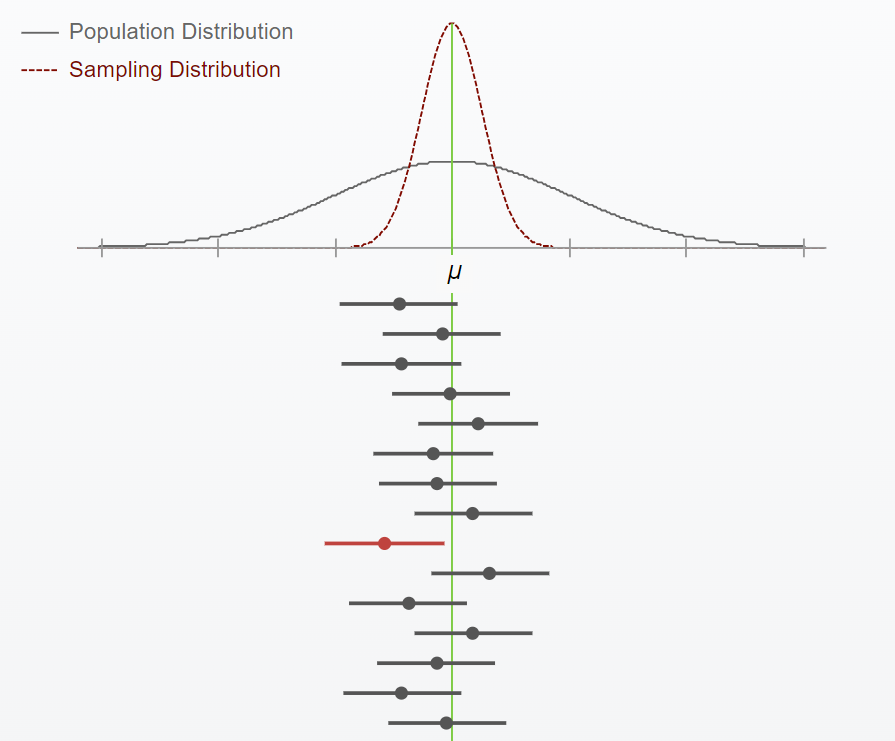
\includegraphics[width=12.43in]{images/endurtekin_oryggisbil} \caption{Endurtekin öryggisbil}\label{fig:unnamed-chunk-2}
\end{figure}

Við getum prófað okkur áfram með forritlingum á netinu, til dæmis \href{http://digitalfirst.bfwpub.com/stats_applet/stats_applet_4_ci.html}{þessum}

Efst á mynd 4.1 sjáum við tvær dreifingar; \textbf{svarta} línan sýnir raunverulega dreifingu í þýði en sú \textbf{rauða} sýnir úrtaksdreifingu þegar dregið er úr þýði með tilviljunarkenndum hætti. \textbf{Græna línan} sem liggur lóðrétt niður myndina endurspeglar raunverulegt þýðismeðaltal. Á línuna hafa verið teiknuð 15 öryggisbil sem gætu fengist. Það er, þarna hafa 15 úrtök verið dregin úr þýðinu með tilviljunarkenndum hætti og öryggisbil reiknað fyrir hvert þeirra. Við sjáum að raunverulegt þýðisgildi liggur innan bilsins í 14 tilfellum af 15. Eitt bilið inniheldur þó ekki þýðisgildið, í þessu úrtaki fellur raunverulegt þýðisgildi utan bilsins.

\begin{center}\rule{0.5\linewidth}{0.5pt}\end{center}

Skoðum nú öryggisbilið sem er rautt. ``\emph{Hverjar eru líkurnar á því að þetta öryggisbil innihaldi raunverulegt þýðisgildi?}'' Það eru engar líkur á því að þýðisgildið sé inn á þessu tiltekna bili. Við getum því ekki litið á eitt öryggisbil og sagt ``\emph{það eru 95\% líkur á að raunverulegt þýðisgildi sé innan bilsins}'' því það hreinlega liggur ekki inn á bilinu.

\textbf{Mikilvægur punktur:} Við getum ekki túlkað einstaka öryggisbil líkt og það séu 95\% líkur á að það innihaldi þýðisgildið. Bilið ýmist inniheldur þýðisgildið, eða ekki. Við vitum ekki hvort okkar öryggisbil sé eitt af þessum 95\% eða meðal þeirra 5\% sem innihalda þýðisgildið ekki. Við vitum bara að \emph{aðferðin} sem við erum að nota muni í 95\% tilfella skila okkur öryggisbili sem inniheldur þýðisgildið.

Skoðum nú efstu tvö öryggisbilin. Á báðum liggur þýðisgildið inn á bilinu; á því fyrsta liggur það við efri mörk bilsins, á því seinna liggur það rétt fyrir miðju.

\textbf{Mikilvægur punktur:} Við vitum ekki hvar á öryggisbilinu þýðisgildið liggur. Við vitum bara að það liggur \emph{sennilega} einhverstaðar innan þess.

\hypertarget{hvauxf0-stjuxf3rnar-breidd-uxf6ryggisbila}{%
\section{Hvað stjórnar breidd öryggisbila?}\label{hvauxf0-stjuxf3rnar-breidd-uxf6ryggisbila}}

\textbf{Úrtaksstærð} Eftir því sem úrtak er stærra --\textgreater{} þeim mun minni breytileiki er í gögnunum --\textgreater{} þeim mun minni óvissa er til staðar --\textgreater{} þeim mun þrengra er bilið.

\begin{itemize}
\tightlist
\item
  Sömuleiðis eftir því sem úrtak er smærra --\textgreater{} þeim mun meiri breytileiki er í gögnunum --\textgreater{} þeim mun meiri óvissa er til staðar --\textgreater{} þeim mun breiðara er bilið.
\end{itemize}

\textbf{Staðalfrávik} Eftir því sem staðalfrávik er lægra --\textgreater{} minni breytileiki í gögnunum --\textgreater{} minni óvissa --\textgreater{} þrengra bil.

\begin{itemize}
\tightlist
\item
  Sömuleiðis; eftir því sem staðalfrávik er hærra --\textgreater{} meiri breytileiki í gögnunum --\textgreater{} meiri óvissa --\textgreater{} víðara bil.
\end{itemize}

\textbf{Öryggið} sem við miðum við, hærra öryggi gefur breiðara bil á meðan lægra öryggi gefur þrengra bil. Skoðum hvers vegna í næsta hluta:

\hypertarget{uxf6ryggiuxf0-uxed-uxf6ryggisbilum}{%
\section{Öryggið í öryggisbilum}\label{uxf6ryggiuxf0-uxed-uxf6ryggisbilum}}

Þó langalgengast sé að nota 95\% öryggisbil er þó hægt að hækka eða lækka öryggið. Hvaða afleiðingar hefur það?

\textbf{90\% öryggisbil:} Ef við notum 90\% öryggi, þá þýðir það að 90\% bila munu innihalda raunverulegt þýðisgildi. Þegar við \textbf{lækkum} öryggið, þá þrengist bilið sömuleiðis. Þetta er vegna þess að kröfurnar eru ekki jafn miklar; aðeins 90\% bilana þurfa að innihalda raunverulegt þýðisgildi svo bilið getur verið þrengra (í samanburði við 95\%ÖB)

\textbf{99\% öryggisbil:} Ef við notum 99\% öryggi, þá þurfa 99\% bilana að innihalda raunverulegt þýðisgildi. Þegar við \textbf{hækkum} öryggið, þá víkkar bilið sömuleiðis. Kröfurnar eru meiri þar sem 99\% bilana þurfa að innihalda raunverulegt þýðisgildi, bilið verður víðara fyrir vikið til að tryggja að þýðisgildið muni vera innan bilsins í 99\% tilfella.

Athugið að þetta þýðir ekki að \textbf{\emph{allar}} úrvinnslur þar sem notast er við 99\% öryggi munu allar gefa víðara bil heldur en þær úrvinnslur þar sem notast er við 95\% öryggi. Ofangreindur samanburður gefur einfaldlega upp afleiðingar þess að breyta öryggi í tiltekinni rannsókn (þ.e. sömu gögn með ólíkt öryggi)

\hypertarget{z-pruxf3f}{%
\chapter{\texorpdfstring{\emph{Z}-próf}{Z-próf}}\label{z-pruxf3f}}

\emph{Z}-próf er einfaldasta marktektarprófið og byggir á normaldreifingu (\emph{z}-dreifing). Prófið gerir ráð fyrir að staðalfrávik þýðis sé þekkt. Við þekkjum auðvitað sjaldnast staðalfrávik þýðis þó vissulega séu til dæmi um það. Til dæmis er greindarvísitala stöðluð og fylgir normaldreifingu (þar sem meðaltalið er 100 og staðalfrávik 15).

Við gætum viljað athuga hvort meðalgreind sálfræðinema við HR sé ólík þekktri meðalgreind; við myndum mæla greind í úrtaki nemenda og gætum síðan notað \emph{z}-próf til að athuga hvort meðalgreind nemendana víki marktækt frá þekktri meðalgreind.

Rifjum upp það sem stóð í kafla 3:

\begin{quote}
Marktektarpróf athugar líkur þess að fá tilteknar úrtakstölur \textbf{ef úrtakið kæmi úr þýði þar sem núlltilgátan er í raun rétt.}
\end{quote}

\begin{itemize}
\item
  Núlltilgáta: Meðalgreind sálfræðinema er sú sama og þekkt meðalgreind. Það er engin munur, munurinn = 0.

  \begin{itemize}
  \tightlist
  \item
    \emph{Til upprifjunar:} marktektarprófið prófar núlltilgátuna!
  \end{itemize}
\item
  Aðaltilgáta: Meðalgreind sálfræðinema er \textbf{ekki} sú sama og þekkt meðalgreind. Það er munur, munurinn er \(\neq\) 0.
\end{itemize}

Við getum vel ímyndað okkur að fá meðalgreind 103 í úrtaki af 15 manns, af tilviljun. Ólíklegra væri að fá meðalgreind 130 í 50 manna úrtaki, af tilviljun (ef núlltilgáta væri rétt og meðalgreind sálfræðinema er 100).

Marktektarprófið athugar líkur þess að fá okkar niðurstöður ef núlltilgátan væri rétt og svarar því spurningunni: ``\emph{EF núlltilgátan er rétt - það er í raun engin munur á meðaltölunum, hverjar væru þá líkur þess að fá svo mikið frávik í 50 manna úrtaki?{}``}

\begin{itemize}
\tightlist
\item
  Ef líkur þess eru \textbf{yfir} 5\% (p \textgreater{} 0,05), þá tölum við um að prófið sé \textbf{ómarktækt} (gefið \(\alpha\) = 0,05).
\item
  Ef líkur þess eru \textbf{undir} 5\% (p \textless{} 0,05), þá tölum við um að prófið sé \textbf{marktækt} (gefið að \(\alpha\) = 0,05).

  \begin{itemize}
  \tightlist
  \item
    Litlar líkur --\textgreater{} ólíklegt að núlltilgáta sé rétt --\textgreater{} marktækt próf --\textgreater{} höfnum núlltilgátu --\textgreater{} höfnum því að það sé enginn munur --\textgreater{} tökum upp aðaltilgátu --\textgreater{} ályktum að það sé munur = meðalgreind sálfræðinema við HR er \textbf{ekki} 100 (þekkt meðalgreind)
  \end{itemize}
\end{itemize}

\hypertarget{kuxed-kvauxf0rat-uxe6fingarduxe6mi}{%
\chapter{Kí-kvaðrat æfingardæmi}\label{kuxed-kvauxf0rat-uxe6fingarduxe6mi}}

Þú átt að athuga hvort það sé samband á milli þess hvort fólk um borð Titanic dóu eftir hárlit þeirra. Neðangreind útlistun gefur þér allar þær upplýsingar sem þú þarft. \emph{Athugaðu að þessar upplýsingar eru klárlega algjört kjaftæði}

Það voru alls 433 farþegar, 210 þeirra dóu og 223 lifðu af. Af þeim sem dóu voru 80 með dökkt hár og 130 með ljóst hár, af þeim sem lifðu af voru 58 með ljóst hár og 165 með dökkt hár.

Þú ættir nú að geta sett upp töflu með rauntíðni og jaðardreifingu, fundið væntitíðni fyrir hver hólf sniðsins og greint frá skilyrtri dreifingu eftir hárlit. Næst ættir þú að geta reiknað kí-kvaðratgildið, athugað marktekt þess, reiknað áhrifastærð og líkindahlutfall. Loks ættir þú að geta sett marktektarniðurstöður fram og gefið túlkun á öllum helstu upplýsingum sem skipta máli.

\hypertarget{rauntuxeduxf0ni-og-jauxf0ardreifing.}{%
\section{Rauntíðni og jaðardreifing.}\label{rauntuxeduxf0ni-og-jauxf0ardreifing.}}

\begin{longtable}[]{@{}llll@{}}
\caption{Fylltu inn í þessa töflu}\tabularnewline
\toprule()
& Hárlitur & & \\
\midrule()
\endfirsthead
\toprule()
& Hárlitur & & \\
\midrule()
\endhead
Dauði? & Dökkur & Ljós & Samtals \\
Dó & ? & ? & ? \\
Lifði af & ? & ? & ? \\
Samtals & ? & ? & ? \\
\bottomrule()
\end{longtable}

Ýttu hér fyrir útfyllta töflu

\begin{longtable}[]{@{}llll@{}}
\toprule()
& Hárlitur & & \\
\midrule()
\endhead
Dauði? & Dökkur & Ljós & Samtals \\
Dó & 80 & 130 & 210 \\
Lifði af & 165 & 58 & 233 \\
Samtals & 245 & 188 & 433 \\
\bottomrule()
\end{longtable}

\hypertarget{vuxe6ntituxeduxf0ni}{%
\section{Væntitíðni}\label{vuxe6ntituxeduxf0ni}}

Finndu væntitíðni fyrir hvert hólf sniðsins. Miðaðu við 2 aukastafi en námundaðu þann síðari ef við á.

\begin{longtable}[]{@{}lll@{}}
\caption{Fylltu inn í þessa töflu}\tabularnewline
\toprule()
& Hárlitur & \\
\midrule()
\endfirsthead
\toprule()
& Hárlitur & \\
\midrule()
\endhead
Dauði? & Dökkur & Ljós \\
Dó & ? & ? \\
Lifði af & ? & ? \\
\bottomrule()
\end{longtable}

Ýttu hér fyrir útfyllta töflu

\begin{longtable}[]{@{}lll@{}}
\toprule()
& Hárlitur & \\
\midrule()
\endhead
Dauði? & Dökkur & Ljós \\
Dó & 118,82 & 91,18 \\
Lifði af & 126,18 & 96,82 \\
\bottomrule()
\end{longtable}

\hypertarget{skilyrt-dreifing.}{%
\section{Skilyrt dreifing.}\label{skilyrt-dreifing.}}

Reiknaðu skilyrta dreifingu eftir hárlit. Hafðu 2 aukastafi en námundaðu þann síðari ef við á.

\begin{longtable}[]{@{}lll@{}}
\caption{Fylltu inn í þessa töflu}\tabularnewline
\toprule()
& Hárlitur & \\
\midrule()
\endfirsthead
\toprule()
& Hárlitur & \\
\midrule()
\endhead
Dauði? & Dökkur & Ljós \\
Dó & ? & ? \\
Lifði af & ? & ? \\
Samtals & ? & ? \\
\bottomrule()
\end{longtable}

Ýttu hér fyrir útfyllta töflu

\begin{longtable}[]{@{}lll@{}}
\toprule()
& Hárlitur & \\
\midrule()
\endhead
Dauði? & Dökkur & Ljós \\
Dó & 32,65\% & 69,15\% \\
Lifði af & 67,35\% & 30,85\% \\
Samtals & 100\% & 100\% \\
\bottomrule()
\end{longtable}

\hypertarget{kuxed-kvauxf0ratgildiuxf0}{%
\section{Kí-kvaðratgildið}\label{kuxed-kvauxf0ratgildiuxf0}}

Reiknaðu kí-kvaðratgildið.

\({\chi}^2=\sum\frac{(Raungildi-Væntigildi)^2}{Væntigildi}\)

Ýttu hér fyrir úrlausn kí-kvaðratgildis

\({\chi}^2 = \frac{(80 - 118,82)^2}{118,82} + \frac{(130 - 91,18)^2}{91,18} + \frac{(165 - 126,18)^2}{126,18} + \frac{(58 - 96,82)^2}{96,82}\)

\({\chi}^2 = 12,68 + 16,53 + 11,95 + 15,56\)

\({\chi}^2 = 56,72\)

Reiknaðu einnig frígráðurnar:

\(df = (r-1)(c-1)\)

Ýttu hér rétta úrlausn frígráða

\(df = (2-1)(2-1)\)

\(df = 1*1\)

\(df = 1\)

\hypertarget{athugauxf0u-marktekt}{%
\section{Athugaðu marktekt}\label{athugauxf0u-marktekt}}

Sýndu mér töfluna

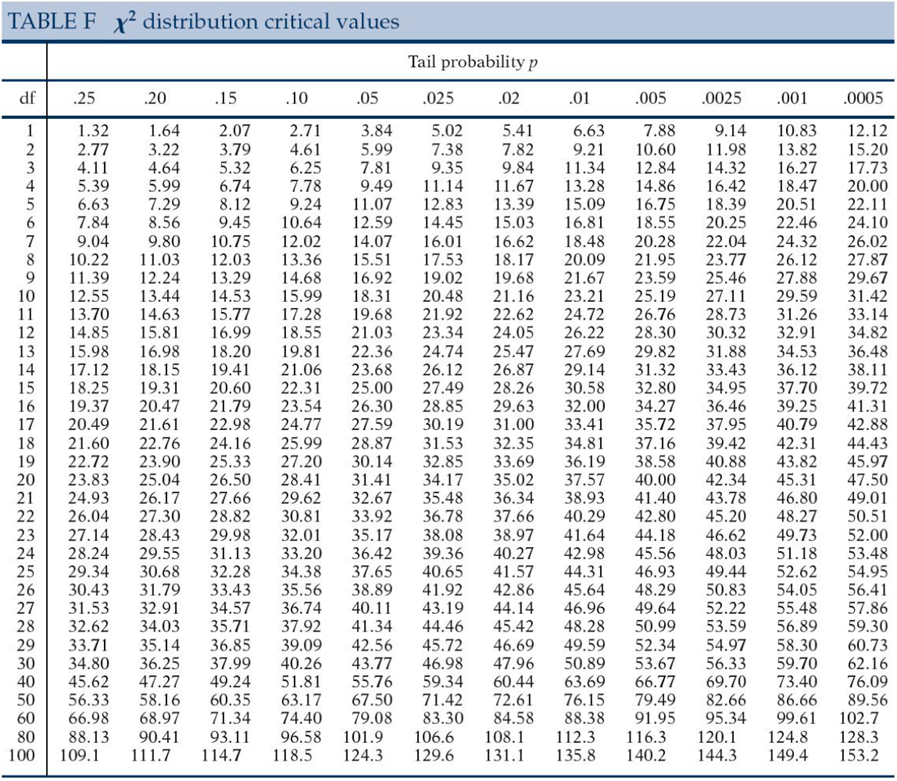
\includegraphics{images/image-2144503272.png}

\textbf{Hvert er vendigildið (critical value)?}

Skilgreining vendigildis:

Vendigildi gefur okkur hvað kí-kvaðratgildi þyrfti að lágmarki að vera til að niðurstaða yrði marktæk.

Vísbending 1:

Þú þarf að vera með frígráður og \(\alpha\) til að finna vendigildið.

Vísbending 2:

Við miðum við \({\alpha}=0,05\) og \({df}=1\)

Rétt svar í töflu:

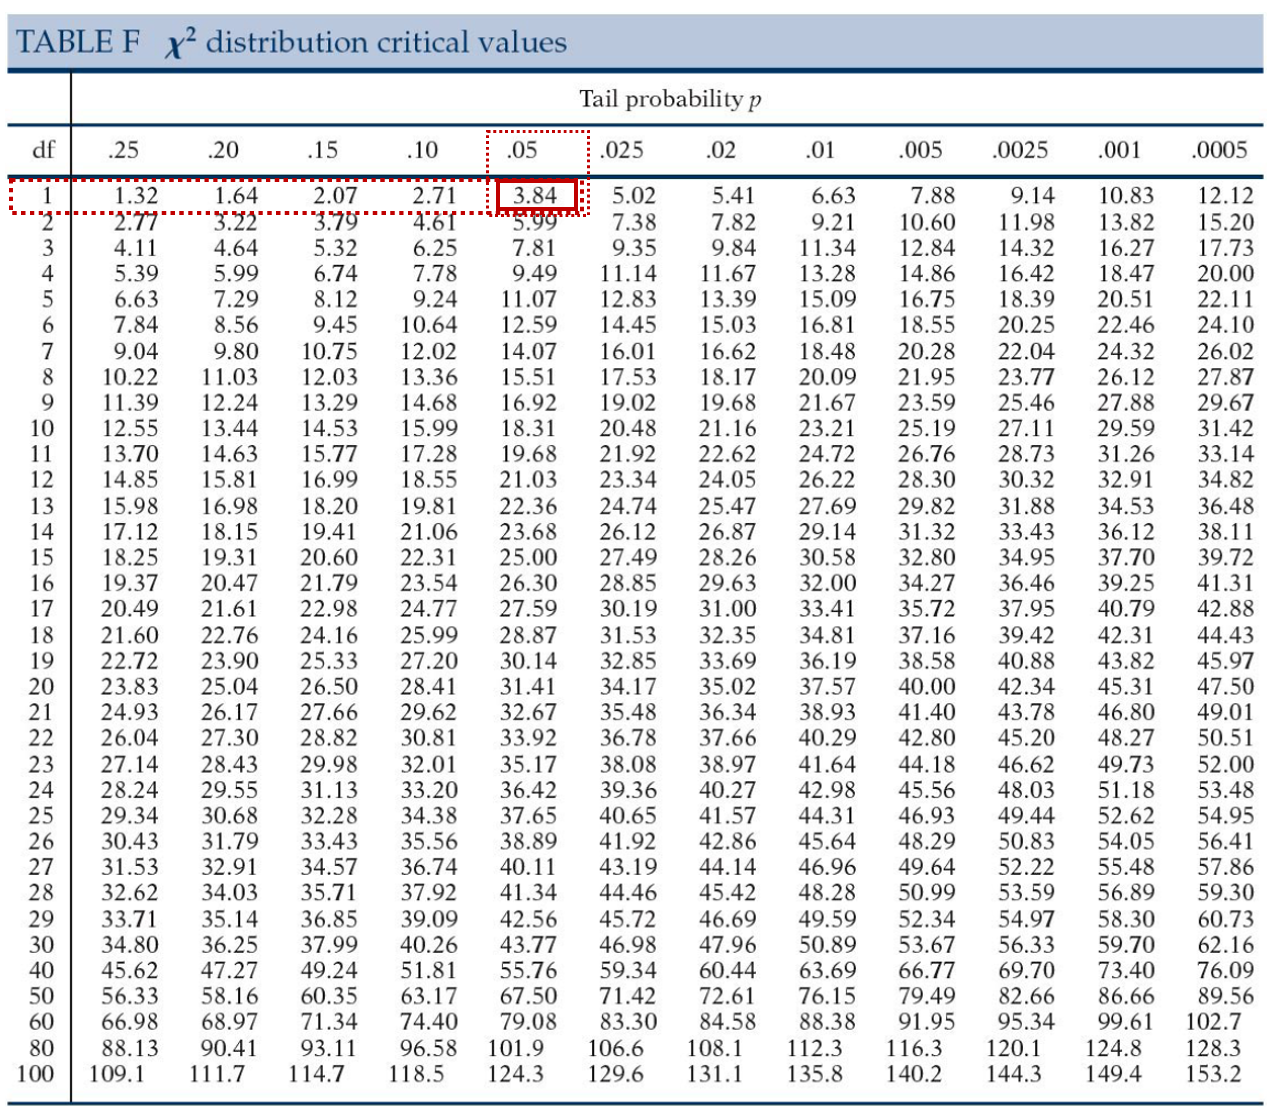
\includegraphics{images/image-490270489.png}

Rétt svar í samfelldu máli:

Kí-kvaðratgildi okkar þyrfti að vera yfir 3,84 til að reynast marktækt.

\textbf{Er prófið marktækt? Hvert er \emph{p}-gildi prófsins?}

Vísbending

þú þarft að vera með frígráður og kí-kvaðratgildi til að finna nákvæmara \emph{p}-gildið

Rétt svar í töflu:

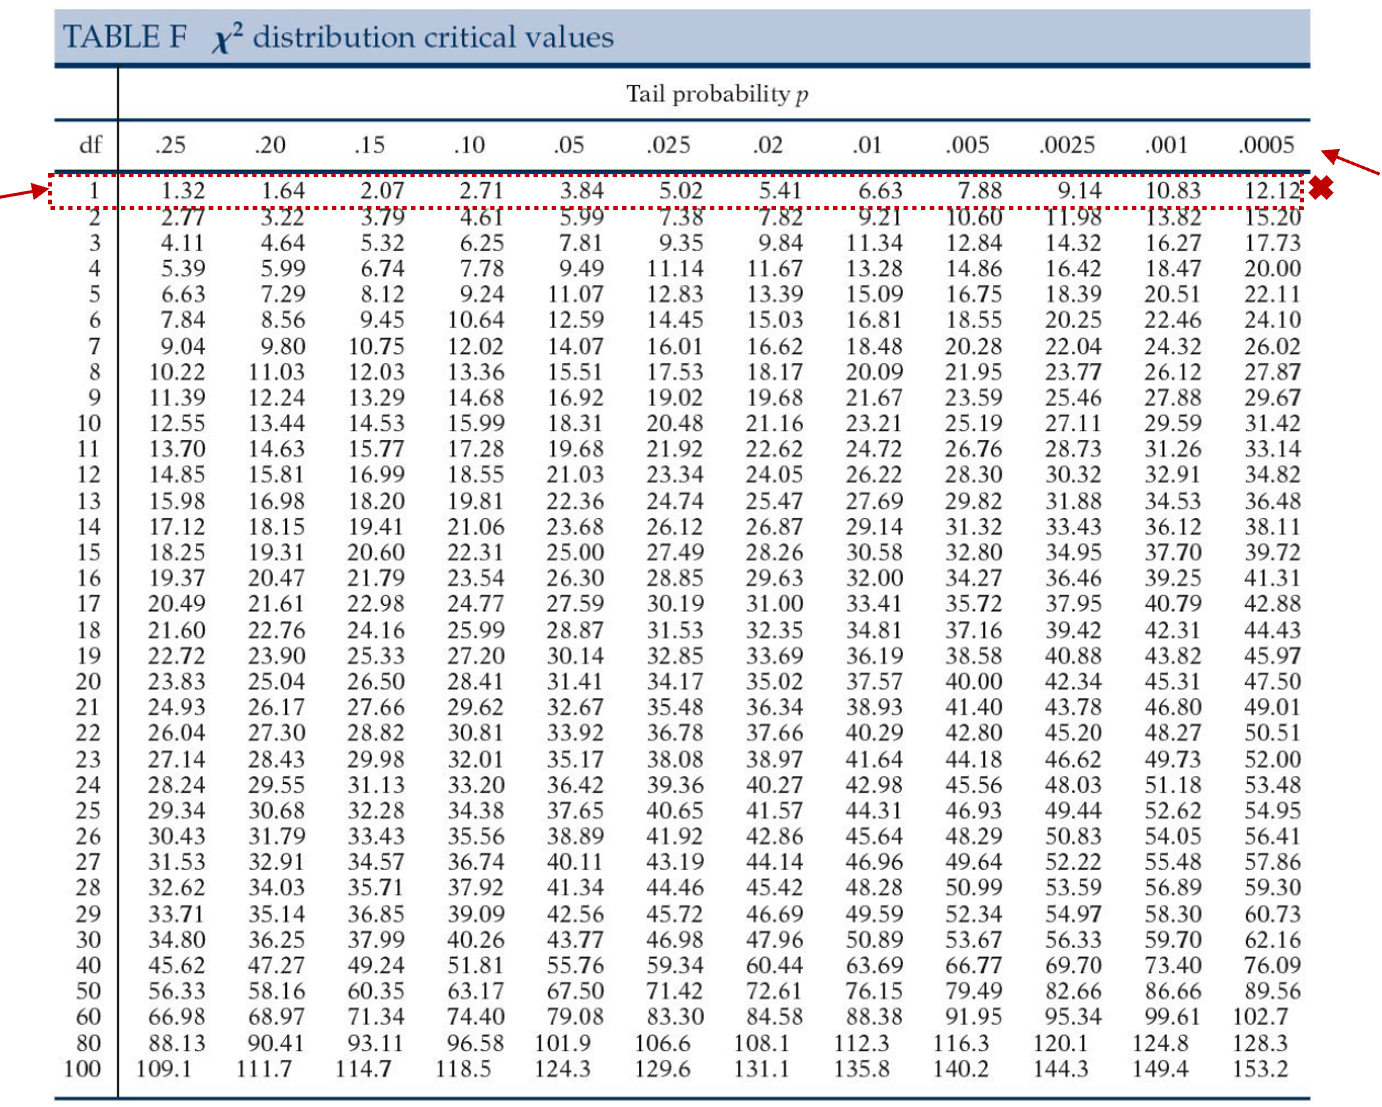
\includegraphics{images/image-580783024.png}

Rétt svar í samfelldu máli:

Já, kí-kvaðratgildið reynist marktækt. Miðað við \({df}=1\) og \({\alpha}=0,05\) þá þyrfti prófstærð okkar að vera 3,84 til að ná marktekt. Kí-kvaðratgildi reyndist hér 56,72 sem liggur utan töflunar, samsvarandi \emph{p}-gildi yrði því undir 0,0005, eða p \textless0,001.

\hypertarget{reikna-uxe1hrifastuxe6ruxf0}{%
\section{Reikna áhrifastærð}\label{reikna-uxe1hrifastuxe6ruxf0}}

Við útreikning áhrifastærðar ætlum við að miða við Cramer's V:

\(V= \sqrt\frac{{\chi}^2}{n * min (r-1, c-1)}\)

Réttur útreikningur

\(V= \sqrt\frac{56,72}{433 * 1}\)

\(V= \sqrt\frac{56,72}{433 * 1}\)

\(V= \sqrt{0,13099}\)

\(V= 0,36192\)

\hypertarget{luxedkindahlutfall}{%
\section{Líkindahlutfall}\label{luxedkindahlutfall}}

Reiknaðu líkindahlutfall sem lýsa því hversu mikið líklegri þeir sem eru ljóshærðir séu að deyja heldur en þeir sem eru dökkhærðir.

Til þessa þarftu að athuga:

\begin{enumerate}
\def\labelenumi{\arabic{enumi}.}
\tightlist
\item
  Reikna líkindi fyrir þá sem eru með ljóst hár og deyja
\item
  Reikna líkindi fyrir þá sem eru með dökkt hár og deyja
\item
  Reikna líkindahlutfall.
\end{enumerate}

Réttur útreikningur og svar

\(Odds_{ljóshærðir sem deyja} = \frac{130}{58} = 2,24\)

\(Odds_{dökkhærðir sem deyja} = \frac{80}{165} = 0,48\)

\(OddsRatio = \frac{Odds_{ljóshærðir sem deyja}}{Odds_{dökkhærðir sem deyja}} = \frac{2,24}{0,48} = 4,6\)

Þeir sem eru með ljóst hár eru 4,6x líklegri til að deyja.

\hypertarget{tuxfalkun-niuxf0urstauxf0na.}{%
\section{Túlkun niðurstaðna.}\label{tuxfalkun-niuxf0urstauxf0na.}}

Hvernig setjum við niðurstöður marktektarprófsins fram á formlegan hátt?

Fylltu inn í eftirfarandi framsetningu:

\({\chi}^2 (?, N = ?) = ?, p = ?\)

Útskýring á spurningamerkjunum

\({\chi}^2 (df, N = fjöldi) = {\chi}^2, p = p-gildi\)

Rétt útfyllt

\({\chi}^2 (1, N = 433) = 56,72, p < 0,001\)

\textbf{Greindu frá niðurstöðunum}

Byrjaðu á því að draga saman upplýsingar úr krosstöflu, taktu niðurstöður síðan saman í stuttu máli þar sem marktektarniðurstöður eru settar fram á formlegan hátt ásamt áhrifastærð og líkindahlutfalli.

Samantekt á krosstöflu

Alls 210 farþegar dóu (48,5\% allra farþega) og af þessum voru 130 ljóshærð (62\% af heild þeirra sem dóu) og 80 dökkhærðir (38\% af heild þeirra sem dóu). Aðrir 233 farþegar dóu ekki (54\% af heildinni) og af þeim voru 58 ljóshærðir (25\% af heild þeirra sem dóu ekki) og 165 voru dökkhærð (71\% af heild þeirra sem dóu ekki). Af þeim sem voru ljóshærðir þá voru 69\% sem dóu og 31\% sem dóu ekki. Af þeim sem voru dökkhærðir voru 33\% sem dóu á móti 67\% sem dóu ekki. Ljóshærðir dóu frekar samanborið við dökkhærða.

Samantekt á niðurstöðum

Marktækt samband var á milli hárlitar farþega um borð Titanic og hvort þau dóu, \({\chi}^2 (1, N = 433) = 56,72, p < 0,001\). Áhrif hárlitar voru miðlungssterk, Cramer\textquotesingle s V = 0,36 en líkindahlutfallið var 4,6 þar sem ljóshærðir voru 4,6x líklegri til að deyja heldur en dökkhærðir.

\hypertarget{breytingar-uxe1-skjali}{%
\chapter{Breytingar á skjali}\label{breytingar-uxe1-skjali}}

\textbf{Útgáfa 1}: 18 janúar

\textbf{Útgáfa 2}: 22 janúar

\begin{itemize}
\item
  \textbf{Breytingar:}

  \begin{itemize}
  \tightlist
  \item
    Vikmörk í dæmi 2 um öryggisbil lagfært - þar voru þau 120.000 en áttu að vera 140.000
  \end{itemize}
\item
  \textbf{Bætt við:}

  \begin{itemize}
  \item
    Kafla 4.1: Mikilvægir eiginleikar öryggisbila
  \item
    Kafla 4.2: Hvað stjórnar breidd öryggisbila?
  \item
    Kafla 4.3: Öryggið í öryggisbilum
  \item
    Kafla 5: Z-próf
  \end{itemize}
\end{itemize}

\textbf{Útgáfa 3}: 11 febrúar

\begin{itemize}
\tightlist
\item
  \textbf{Bætt við}: Kafli 7: æfingardæmi fyrir kí-kvaðrat.
\end{itemize}

  \bibliography{book.bib,packages.bib}

\end{document}
